\documentclass{article}
\usepackage{verbatim}
\usepackage{moreverb}
\usepackage{url}
\usepackage{amsmath}
\usepackage{color}
\usepackage{appendix}
\author{Vadim Zaliva, lord@codeminders.com}
\date{2010}
\title{Dataflow Approach to Data Processing in Hadoop with HAMAKE}
\usepackage{graphicx}
\usepackage{listings}
\usepackage{rotating}
\usepackage[colorlinks=true,bookmarks=true,pdfauthor={Vadim Zaliva lord@crocodile.org},
            pdftitle={Dataflow Approach to Data Processing in Hadoop with HAMAK},
            pdftex]{hyperref}

% graphviz.tex
% originally written by Derek Rayside, November 2003
% following an idea that Daniel Jackson implemented in his Tagger program
%
% parameters to \digraph:
% 1 - parameters for \includegraphics (optional; default value is "scale=1")
% 2 - name of the digraph
% 3 - body of the digraph

\newcommand{\digraph}[3][scale=1]{
    \newwrite\dotfile
    \immediate\openout\dotfile=#2.dot
    \immediate\write\dotfile{digraph #2 {\string#3}}
    \immediate\closeout\dotfile
    \IfFileExists{#2.ps}
        % the postscript exists: include it
        { \includegraphics[#1]{#2} }
        % the postscript doesn't exist: tell the user how to create it
        { \fbox{ \begin{tabular}{l}
            The file \texttt{#2.ps} hasn't been created from
            \texttt{#2.dot} yet. \\
            Run `\texttt{dot -Tps -o #2.ps #2.dot}' to create it. \\
            Here is a \textsf{bash} loop to process all \textsf{dot} files
            in the current directory: \\
            \texttt{
            for f in *.dot do ; 
            dot -Tps -o \$\{f\%dot\}ps \$f ; 
            done
            }
            \end{tabular}}
        }
}


\begin{document}
\lstset{language=XML,basicstyle=\tiny,markfirstintag=true,numbers=left, numberstyle=\tiny}

\maketitle

\begin{abstract}
  Most non-trivial data processing scenarios with Hadoop typically
  require more than one MapReduce job. Usually such processing is
  data-driven, with the data funneled through a sequence of jobs. The
  processing model could be presented in terms of dataflow
  programming. It could be expressed as a directed graph, with
  datasets as nodes. Each edge indicates a dependency between two or
  more datasets and is associated with a processing instruction
  (Hadoop MapReduce job, PIG Latin script or an external command),
  which produces one dataset from the others. Using fuzzy timestamps
  as a way to detect when a dataset needs to be updated, we can
  calculate a sequence in which the jobs need to be executed to bring
  all datasets up to date. Jobs for updating independent datasets
  could be executed concurrently, taking advantage of your Hadoop
  cluster's full capacity. The dependency graph may even contain
  cycles, leading to dependency loops which could be resolved using
  dataset versioning.

  These ideas inspired the creation of HAMAKE utility. We tried
  emphasizing data and allowing the developer to express one's goals
  in terms of dataflow (versus workflow). Data dependency graph is
  expressed using just two data flow instructions: fold and foreach
  providing a clear processing model, similar to MapReduce, but on a
  dataset level. Another design goal was to create a simple to use
  utility that developers can start using right away without complex
  installation or extensive learning. We think we have been able to
  achieve these goals and the utility we have created has been
  successfully used in real-life large scale Hadoop data processing
  projects. 
\end{abstract}

\section{Introduction}

MapReduce model introduced by Google\cite{dean2008map} allows
processing of large data amounts. Hadoop\cite{bialecki2005hadoop} is
popular open-source implementation of MapReduce.

Hadoop is usually used to proccess big amounts of data. The
consequence of this is that even trivial tasks are generally I/O-bound
\cite{hadoopattwitter},\cite{hs2010hadoopbench} which put special
emphasis on incremental processing.

\section{Processing Model}

Hamake operates on \textit{filesets} which consists of indvidual
\textit{files}. Fileset defines group of files, residing on filesystem
accessible from Hadoop task (usually DFS). \textit{Dataflow
  transformation rules (DTR)} specify operations which could take some
files or filesets as inputs (or dependecies) and possibly produce
other filesets as output.

\subsection{Dependecy Resolution}

If file \textit{A} is listed as input of a DTR, and file \textit{B}
listed as output of the same DTR, it is said that \textit{``B depends
  on A''}. Hamake is using file time stamps for dependency
calculation. A time stamp of a file is date and time when it was last
modified.  In hamke world, file system directory or folder is also a
file, and has its own time stamp. DTR outputs said to be \textit{up to
  date} if minimal time stamp on all outputs is greater or equal than
maximum timestamp on all inputs (and dependency inputs).

hamake attempts to ensure that all DTR outputs are up to
date\footnote{we do not try to ensure that files which are not listed
  as DTR outputs are up to date, becase we have no way to update
  them}. To do so it builds a \textit{dependency graph}. This graph
have files or filesets as vertices and DTRs as edges. (TODO: is it DAG?)

Then, the graph reduction algorithms shown on Figure~\ref{fig:grred}
is performed.

\begin{figure}[htp]
\centering
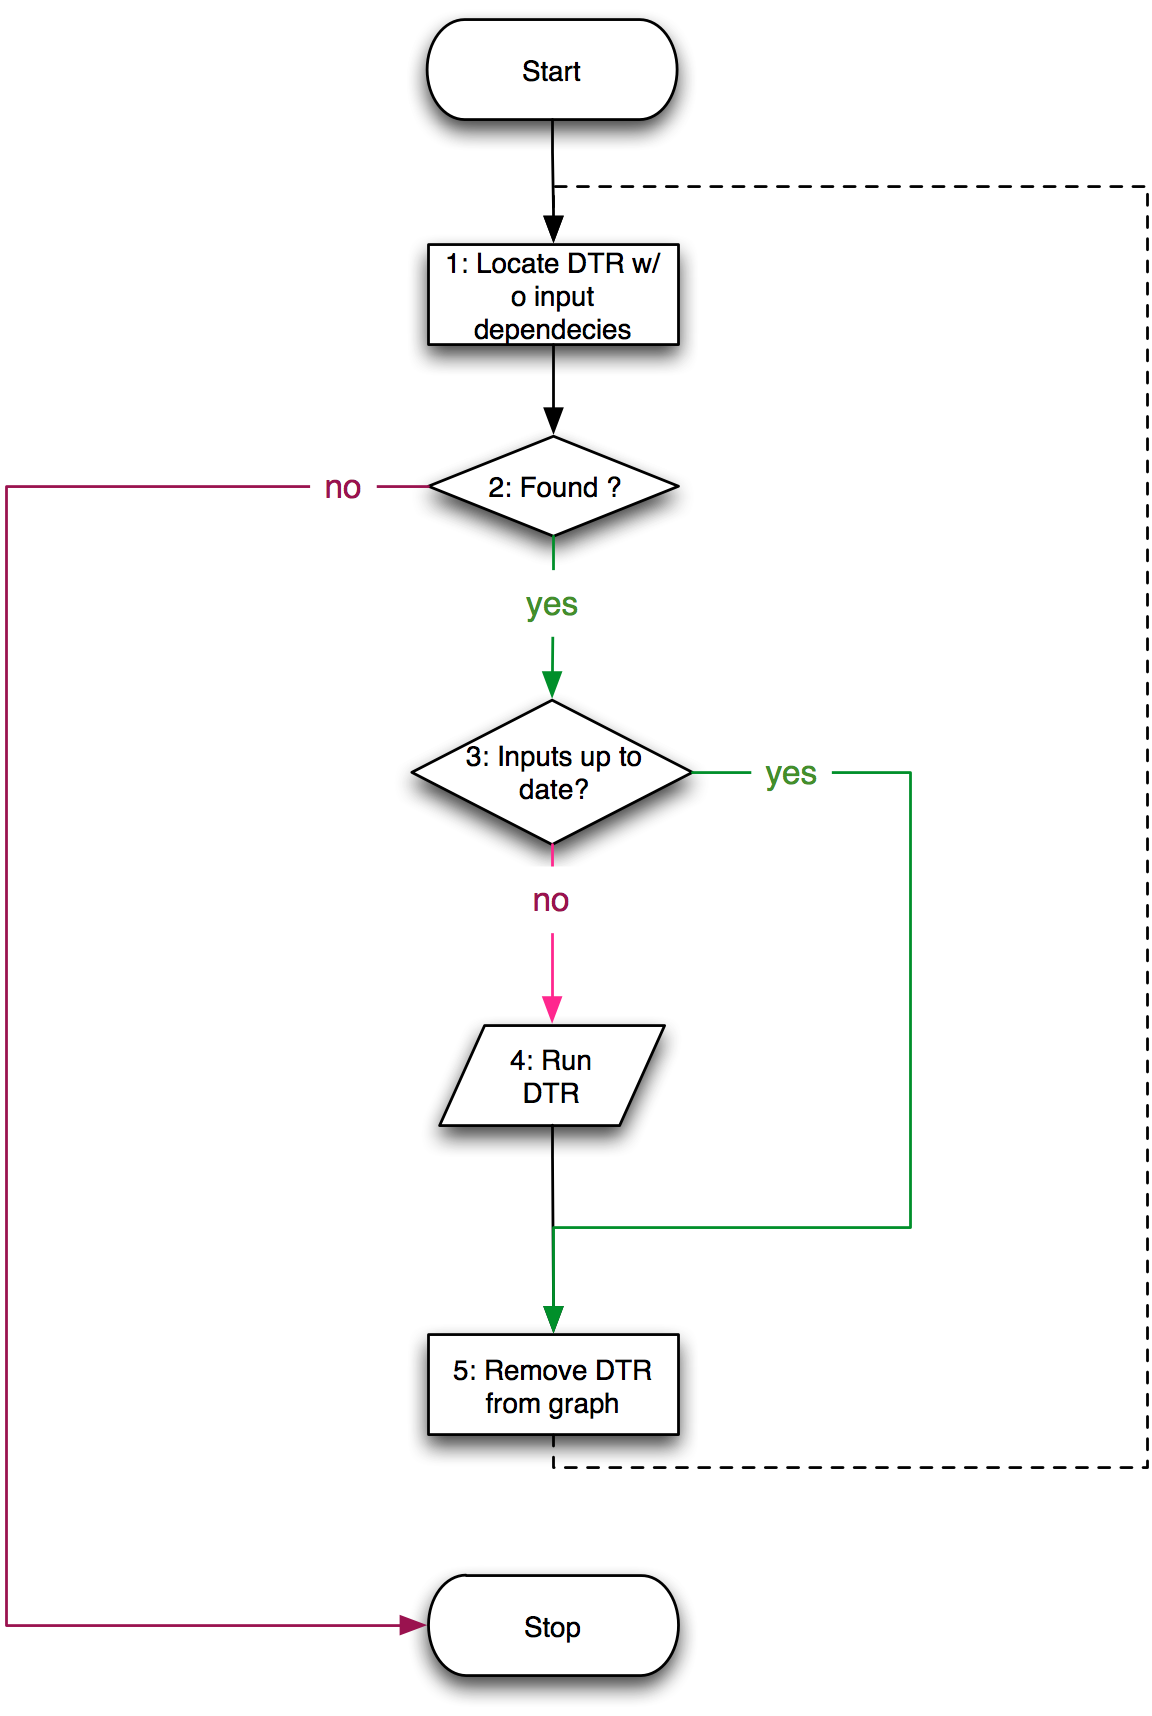
\includegraphics[width=10cm]{GraphReduction.png}
\caption{hamake dependency graph reduction algorithm}
\label{fig:grred}
\end{figure}

Some steps could be executed in parallel: if more than one DTR without
input dependencies is found on step 1, subsequent steps 2-5 could be
executed for each discovered DTR in parallel.

TODO: error handling in step 4?

Essentially, this a version of Kahn's
algorithm\cite{kahn1962topological}, implementing topological
ordering\cite{wiki:topsort}.


\subsubsection{Cyclic Dependences}

Cyclic dependences has to be avoided, because workflow contaning them
is not guaranteed to terminate. (TODO: could not be presented as DAG?)
Implicit checks are perfomed during reading hamakefile and building
dependency graph. If a cycle is detected, it is reported as an
error. So the dependency graph used by hamake is \textit{directed
  acyclic graph}.

However hamake supports a limited scenario of interative processing, where
some output of one iteration are used as an input in the next one. We
do not support more general case of \textit{fixed point} iterative
calculations: each run of hamake is a signle pass. This mechanism
is implemented via hamake feature called \textit{generations}. Each
input or output file could be optionally marked with \emph{generation}
attribute. Same file with with different generation numbers is treated
as different vertex is dependency graph. (TODO: elaborate)

\subsection{Path Transformation Operations}

TBD

\section{Implementation}

A Python-language prototype of \textit{hamake} was developed in late
2008 and has been used on a daily basis ever since. Based on our
experience with the prototype, we built a new version of the
product. Re-written from scratch in Java, the new version has many
improvements like streamlined syntax of a dataflow definition file,
Amazon EMR support and others.

TODO: mention open source


\section{Scheduler}

The design goal of hamake scheduler to perform all required
calculations in shortest possible time. Obviously to achive this it
should aim for maximal cluster utilization, performing as many
calculations in parallel as possible.

There are three factors driving scheduling loginc: DTR dependencies,
files, and Hadoop tasks.

On highest level DTR dependencies determine sequence of DTRs jobs
being launched. In case of \emph{fold} DTR, normally a single Hadoop
job, PIG script or shell command is launched. However in case of
\emph{foreach} DTRs, an additional level of parallelism could be
achived, as individual jobs will be launched for each input file.

\begin{figure}[htp]
\centering

\includegraphics[width=6cm]{twofold.png}
\caption{Simple \emph{fold} DTR}
\label{fig:fold1}
\end{figure}

In example shown on Figure~\ref{fig:fold1}, since fileset \textit{B}
depends on all files in fileset \textit{A}, there are not many
opportunities to for parallel execution and \emph{fold} DTR is
executued as as single job. At first glance, two dependent
\emph{foreach} shown in Figure~\ref{fig:foreach1} DTRs looks similar.

\begin{figure}[htp]
\centering

\includegraphics[width=7cm]{twoforeach.png}
\caption{Simple \emph{foreach} DTR}
\label{fig:foreach1}
\end{figure}

However \emph{foreach} DTRs works by mapping individual files in
fileset \textit{A} to files in fileset \textit{B}. Assuming that
fileset \textit{A} consists of 3 files: \textit{a1}, \textit{a2},
\textit{a3} the the dependency graph could be represented as shown on
Figure~\ref{fig:foreach2}.

\begin{figure}[htp]
\centering
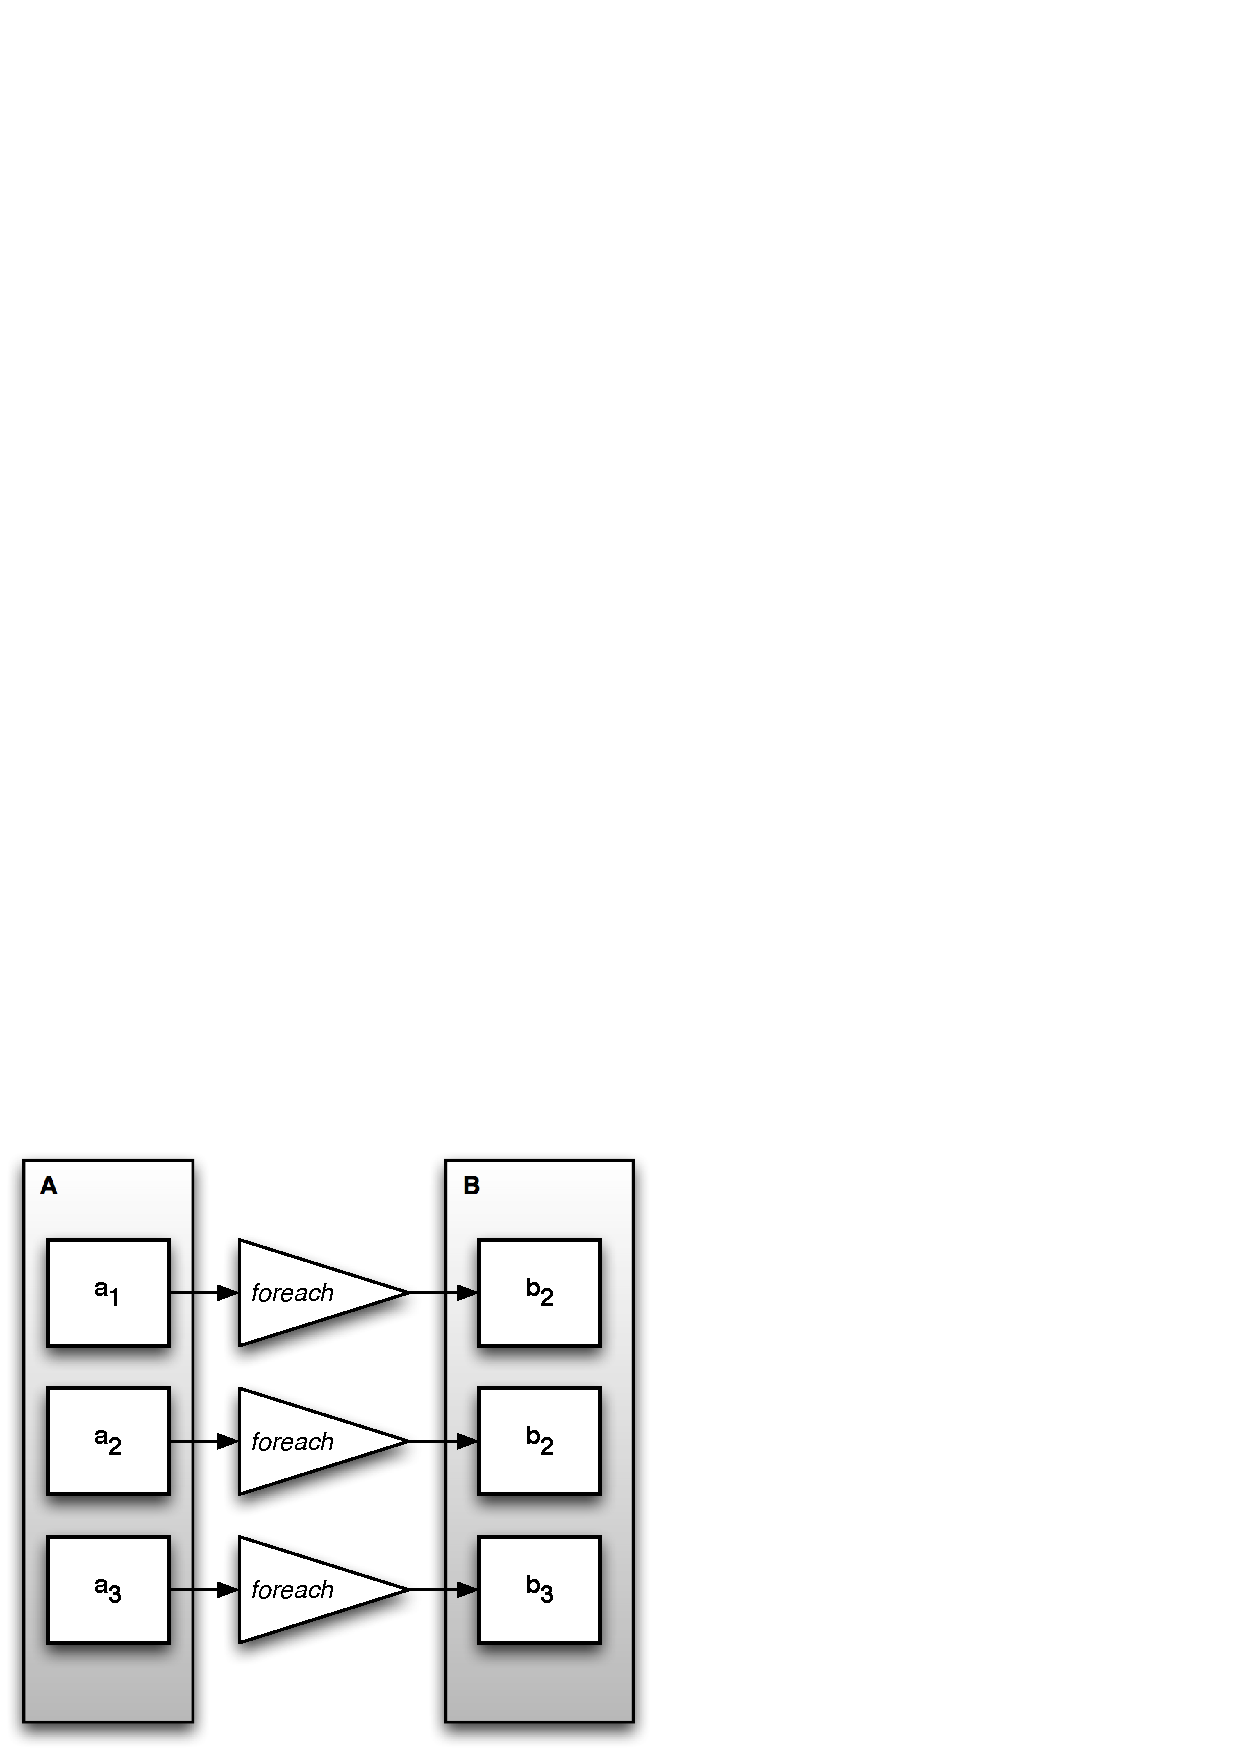
\includegraphics[width=7cm]{twoforeachp.png}
\caption{Decomposition of \emph{foreach} DTR}
\label{fig:foreach2}
\end{figure}

In this case we have an opportunity to execute three jobs in parallel.

Unltimately, the Hadoop cluster capacity is defined in terms of number
of \textit{map slots} and \textit{reduce slots}.  DTR lauches Hadoop
job (either directly as defined by \emph{mapreduce} instruction or via
PIG script, single job will spawn one or more \emph{mapper} and
\emph{reducer} tasks, each taking one respecive slot. Number of
mappers and reducers lauched depends on many factors: size of DFS
block, Hadoop general settings, \emph{JobConf} settings for particular
job are among them. In general, hamake does not have an neither
visibility nor control over most of these factors, so the hamake
scheduler currently does not deal with invidual tasks. It knows only
about data files and spawned Hadoop jobs.

\section{Related Work}

Table~\ref{table:1} below attempts to compare Hamake and similar
workflow engines for Hadoop
(\href{http://github.com/tucu00/oozie1}{Oozie},
\href{http://sna-projects.com/azkaban/}{Azkaban},
\href{http://www.cascading.org/}{Cascading}) based on some key
features. Although all of these systems could be used to solve similar
problems, they differ significantly in design, philosophy, target user
profile, usage scenarios, etc.  So our feature-wise comparison is in
no way conclusive. Please use it as a guideline, but read respective
systems documentation to understand better which one is more suitable
for your problem.

\begin{sidewaystable}
  \begin{tabular}{ | p{3cm} || l | l | l | l |}
    \hline
    \textbf{Feature} & \textbf{hamake} & \textbf{Oozie} & \textbf{Azkaban} & \textbf{Cascading} \\
    \hline
    Workflow discription language & XML & XML (xPDL based) & text file with key/value pairs & Java API \\
    Dependencies mechanism & data-driven & explicit & explicit & explicit \\
    Requires Servlet/JSP container & No & Yes & Yes & No \\
    Allows to track a workflow progress & console/log messages & web page & web page & Java API \\
    Ability to schedule a Hadoop job execution at given time & no & yes & yes & yes \\
    Execution model & command line utility & daemon & daemon & API \\
    Allows to run Pig Latin scripts & yes & yes & yes & yes \\
    Event notification & no & no & no & yes \\
    Requires installation & no & yes & yes & no \\
    Supported Hadoop version & 0.18+ & 0.20+ & currently unknown & 0.18+ \\
    Retries & no & at workflow node level & yes & yes \\
    Ability to run arbitrary commands & yes & yes & yes & yes \\
    Can be run on  Amazon EMR & yes & no & currently unknown & yes \\
    \hline
  \end{tabular}
  \caption{Feature comparison of popular Hadoop workflow engines }
  \label{table:1}
\end{sidewaystable}

Below are some notes, discussing some key differences between hamake
and some other popular products:

\subsection{Cascading}

In short: Cascading is an API, while hamake is an utility. Some differences:
\begin{itemize}
\item hamake does not require any custom programming. It helps to automate running your existing Hadoop tasks and PIG scripts
\item You can use hamake to automate tasks written in other languages, for example using \textit{Hadoop streaming}
\end{itemize}

\subsection{Oozie and Azkaban}

Oozie and Azkaban are server-side systems that have to be installed
and run as a service. Hamake is a lightweight client-side utility that
does not require installation and has very simple syntax for workflow
definition.  Most importantly, Hamake is built based on dataflow
programming principles - your Hadoop tasks execution sequence is
controlled by the data.
 

\section{Future Work}

Better integration with Hadoop schedulers (Fair Scheduler, Capacity
Scheduler, etc.).

\nocite{*}
\bibliography{hamake}
\bibliographystyle{unsrt}

\end{document}

